\PassOptionsToPackage{dvipsnames,svgnames,x11names}{xcolor}
\documentclass[tikz,border=8pt]{standalone}
\usetikzlibrary{arrows.meta,positioning,calc,shapes,shadows,decorations.pathmorphing,shapes.geometric,backgrounds,decorations.markings,decorations.pathreplacing,decorations.text,fit,shapes.misc,shapes.arrows,matrix,bending,3d,chains,intersections,shapes.symbols,svg.path,shapes.multipart,snakes,shapes.callouts,angles,quotes}
\providecolor{gold}{RGB}{212,175,55}
\providecolor{silver}{RGB}{192,192,192}
\providecolor{bronze}{RGB}{205,127,50}
\providecolor{darkblue}{RGB}{0,0,139}
\providecolor{lightblue}{RGB}{173,216,230}
\providecolor{darkgreen}{RGB}{0,100,0}
\providecolor{lightgreen}{RGB}{144,238,144}
\providecolor{darkred}{RGB}{139,0,0}
\providecolor{navy}{RGB}{0,0,128}
\providecolor{skyblue}{RGB}{135,206,235}
\providecolor{beige}{RGB}{245,245,220}
\providecolor{cream}{RGB}{255,253,208}
\usepackage{amsmath}
\usepackage{amssymb}
\usepackage{fontawesome5}
\usetikzlibrary{fadings,shadows.blur,patterns,patterns.meta}

\providecolor{gold}{RGB}{212,175,55}
\providecolor{silver}{RGB}{192,192,192}
\providecolor{bronze}{RGB}{205,127,50}
\providecolor{darkblue}{RGB}{0,0,139}
\providecolor{lightblue}{RGB}{173,216,230}
\providecolor{darkgreen}{RGB}{0,100,0}
\providecolor{lightgreen}{RGB}{144,238,144}
\providecolor{darkred}{RGB}{139,0,0}
\providecolor{navy}{RGB}{0,0,128}
\providecolor{skyblue}{RGB}{135,206,235}
\providecolor{beige}{RGB}{245,245,220}
\providecolor{cream}{RGB}{255,253,208}
\usepackage{amsmath}
\usepackage{amssymb}
\usepackage{fontawesome5}

\usepackage{tikz}
\usepackage{xcolor}

% --- COLOR PALETTE ---
\definecolor{accentblue}{RGB}{41, 128, 185}
\definecolor{accentred}{RGB}{192, 57, 43}
\definecolor{accentgreen}{RGB}{39, 174, 96}
\definecolor{accentpurple}{RGB}{142, 68, 173}
\definecolor{textdark}{RGB}{44, 62, 80}
\definecolor{codebg}{RGB}{40, 44, 52}
\definecolor{codetext}{RGB}{171, 178, 191}

\begin{document}
\begin{tikzpicture}

% ==============================================================================
% 1. BACKGROUND CANVAS
% ==============================================================================
\fill[white] (0, -1) rectangle (20, 24);

% ==============================================================================
% 2. TITLE & INTENT (Y: 21 to 24)
% ==============================================================================
\node[font=\fontsize{36}{42}\selectfont\bfseries\color{textdark}, anchor=north] at (10, 23.5) {Art Direction};
\node[font=\Large\color{textdark!80}, anchor=north, align=center, text width=16cm] at (10,21.3902) {Intent: Deliver a \textbf{differently cropped or modified} image based on the context.\\The primary goal is \textbf{visual clarity} and keeping the subject prominent on any screen size.};

% ==============================================================================
% 3. MASTER IMAGE MACRO (Photorealistic Landscape & Lifelike Silhouette)
% ==============================================================================
\newcommand{\drawMasterImage}{
    % Sky Gradient
    \shade[top color=cyan!25!blue!20, bottom color=orange!20!yellow!15] (3, 13) rectangle (17, 17);

    % Glowing Sun (Positioned at X=6.5, strictly excluded from Tablet Crop X>=8)
    \shade[inner color=yellow!90!orange, outer color=yellow!10!orange!0] (6.5, 15.7) circle (0.9);
    \fill[yellow!90!white] (6.5, 15.7) circle (0.35);

    % Background Mountain Ridge
    \shade[top color=white!90!gray, bottom color=blue!20!gray!60] (3, 13) -- (4.2, 15.0) -- (5.8, 14.1) -- (7.6, 15.8) -- (9.6, 14.0) -- (11.4, 15.5) -- (14.0, 13) -- cycle;

    % Midground Realistic Mountains with Snow Caps
    \shade[top color=white, bottom color=gray!60] (6.5, 13) -- (8.5, 16.2) -- (10.5, 13) -- cycle;
    \shade[top color=white, bottom color=gray!50] (10.5, 13) -- (12.2, 15.4) -- (14.2, 13) -- cycle;
    \shade[top color=white, bottom color=gray!40] (8.5, 16.2) -- (7.8, 15.2) -- (9.2, 15.1) -- cycle;
    \shade[top color=white, bottom color=gray!40] (12.2, 15.4) -- (11.6, 14.7) -- (12.8, 14.6) -- cycle;

    % Rolling Valley Greenery
    \shade[top color=green!50!teal!50, bottom color=green!30!black!80] (3, 13) to[out=5, in=185] (10, 13.6) to[out=5, in=175] (17, 13.2) -- (17, 13) -- (3, 13) -- cycle;

    % Foreground Cliff (Focal Point on the right)
    \shade[top color=gray!40!brown!70, bottom color=black!90] (14.0, 13) -- (14.6, 14.3) to[out=15, in=180] (15.6, 15.1) -- (17, 15.1) -- (17, 13) -- cycle;

    % Cliff Rock Strata Texture
    \draw[black!60, line width=0.8pt] (14.7, 14.0) to[out=15, in=190] (16.9, 14.6);
    \draw[black!50, line width=0.6pt] (15.0, 13.5) to[out=10, in=195] (17.0, 13.9);

    % Lifelike Hiker Vector Silhouette
    \begin{scope}[shift={(15.8, 14.5)}, scale=0.35]
      \fill[black] (0.3, 2.5) circle (0.35); % Head
      \fill[black] (0.1, 1.0) .. controls (-0.2, 1.5) and (0.0, 2.2) .. (0.3, 2.2) .. controls (0.6, 2.2) and (0.7, 1.5) .. (0.6, 1.0) -- cycle; % Torso
      \fill[black!85] (-0.4, 1.2) .. controls (-0.6, 1.6) and (-0.4, 2.1) .. (-0.1, 2.1) -- (0.1, 1.2) -- cycle; % Backpack
      \draw[black, line width=3.5pt, line cap=round] (0.2, 1.1) -- (0.0, 0.5) -- (-0.3, -0.2); % Left Leg
      \draw[black, line width=3.5pt, line cap=round] (0.5, 1.1) -- (0.6, 0.4) -- (0.8, -0.2); % Right Leg
      \draw[black, line width=2.5pt, line cap=round] (0.4, 1.9) -- (0.7, 1.3) -- (1.1, 1.4); % Arm
      \draw[black, line width=1.5pt, line cap=round] (1.1, 1.8) -- (0.9, -0.3); % Hiking pole
    \end{scope}
}

% ==============================================================================
% 4. MASTER CANVAS & CROP BOXES (Top Section, Y: 13 to 19)
% ==============================================================================

% Art Director Callout
\node[font=\Huge, text=accentpurple] at (1.0, 16.0) {\faCrop};
\node[font=\small\bfseries, text=textdark, align=center, text width=2.5cm] at (1.0, 14.8) {Art Director\\determines\\best crops\\per screen};
\draw[-Stealth=3mm, thick, accentpurple, dashed] (2.3, 15.0) -- (2.8, 15.0);

% Master Scene Container with Shadow, Clipping, and Technical Grid Overlay
\begin{scope}
    \fill[white, drop shadow={shadow xshift=2pt, shadow yshift=-4pt, shadow opacity=30}] (3, 13) rectangle (17, 17);
    \begin{scope}
        \clip (3, 13) rectangle (17, 17);
        \drawMasterImage
        % Subtle translucent technical grid lines
        \draw[step=0.5cm, gray!60, opacity=0.2, very thin] (3, 13) grid (17, 17);
    \end{scope}
    \draw[line width=1.2pt, textdark!80] (3, 13) rectangle (17, 17);
\end{scope}

% Desktop Crop Box (Green) - Wide Panorama (Outer boundary)
\draw[accentgreen, dashed, line width=2pt] (3.0, 12.7) rectangle (17.3, 17.3);
\node[fill=accentgreen, text=white, font=\footnotesize\bfseries, inner sep=4pt, anchor=south west, rounded corners=1pt] at (3.0, 17.3) {Desktop Crop};

% Tablet Crop Box (Blue) - Left-trimmed Panorama (Middle boundary)
\draw[accentblue, dashed, line width=2pt] (8.0, 12.85) rectangle (17.15, 17.15);
\node[fill=accentblue, text=white, font=\footnotesize\bfseries, inner sep=4pt, anchor=south west, rounded corners=1pt] at (8.0, 17.15) {Tablet Crop};

% Mobile Crop Box (Red) - Focus on Subject (Inner boundary)
\draw[accentred, dashed, line width=2pt] (13.0, 13.0) rectangle (17.0, 17.0);
\node[fill=accentred, text=white, font=\footnotesize\bfseries, inner sep=4pt, anchor=south west, rounded corners=1pt] at (13.0, 17.0) {Mobile Crop};

% ==============================================================================
% 5. ZERO-INTERSECTION ROUTING (The Flow Arrows)
% ==============================================================================
% Desktop (Green): Center of Desktop Crop (10.0, 12.7) to Top of Desktop Device (4.0, 9.2)
\draw[line width=1.5pt, accentgreen, -Stealth=3mm, out=-90, in=90] (10.0, 12.7) to (4.0, 9.2);

% Tablet (Blue): Center of Tablet Crop (12.5, 12.85) to Top of Tablet Device (10.0, 9.2)
\draw[line width=1.5pt, accentblue, -Stealth=3mm, out=-90, in=90] (12.5, 12.85) to (10.0, 9.2);

% Mobile (Red): Center of Mobile Crop (15.0, 13.0) to Top of Mobile Device (16.0, 9.2)
\draw[line width=1.5pt, accentred, -Stealth=3mm, out=-90, in=90] (15.0, 13.0) to (16.0, 9.2);

% ==============================================================================
% 6. DEVICES WITH ACCURATE MATHEMATICAL CLIPPING (Middle Section, Y: 4.8 to 9.2)
% ==============================================================================

% --- [LEFT] DESKTOP DEVICE (Center X: 4.0) ---
% Base / Stand
\fill[gray!40, rounded corners=1.5pt] (3.2, 5.3) rectangle (4.8, 5.5);
\fill[gray!55] (3.7, 5.5) -- (3.8, 6.5) -- (4.2, 6.5) -- (4.3, 5.5) -- cycle;
% Monitor Outer Body
\fill[black!85, rounded corners=2.5mm, drop shadow={shadow xshift=2pt, shadow yshift=-4pt, shadow opacity=30}] (1.0, 6.5) rectangle (7.0, 9.2);
% Browser Window Header
\fill[gray!30] (1.2, 8.6) rectangle (6.8, 9.0);
\fill[red!70!black] (1.45, 8.8) circle (0.06);
\fill[yellow!80!black] (1.7, 8.8) circle (0.06);
\fill[green!70!black] (1.95, 8.8) circle (0.06);
\fill[white, rounded corners=1pt] (2.3, 8.68) rectangle (6.4, 8.92);
\node[font=\tiny, text=gray!70, anchor=west] at (2.4, 8.8) {desktop-view};
% Screen Content (Mathematically Mapped with scale=0.4)
\begin{scope}
    \clip (1.2, 7.0) rectangle (6.8, 8.6);
    \begin{scope}[shift={(1.2, 7.0)}, scale=0.4, shift={(-3, -13)}]
        \drawMasterImage
    \end{scope}
    \fill[white, opacity=0.08] (1.2, 7.0) -- (6.8, 8.6) -- (6.8, 7.0) -- cycle;
\end{scope}
\node[font=\footnotesize\bfseries, text=textdark, align=center] at (4.0956,4.4561) {\faEye \ Vast Landscape\\desktop-wide.jpg};

% --- [CENTER] TABLET DEVICE (Center X: 10.0) ---
% Aluminum Outer Frame
\fill[gray!25, rounded corners=3mm, drop shadow={shadow xshift=2pt, shadow yshift=-4pt, shadow opacity=30}] (7.8, 6.5) rectangle (12.2, 9.2);
% Inner Black Bezel
\fill[black!90, rounded corners=2mm] (8.0, 6.7) rectangle (12.0, 9.0);
% Front Camera Lens
\fill[gray!60] (10.0, 9.1) circle (0.06);
\fill[blue!40!black] (10.0, 9.1) circle (0.03);
% Screen Content (Mathematically Mapped with scale=0.4, X=8 aligned to left edge)
\begin{scope}
    \clip[rounded corners=1mm] (8.2, 7.0) rectangle (11.8, 8.6);
    \begin{scope}[shift={(8.2, 7.0)}, scale=0.4, shift={(-8, -13)}]
        \drawMasterImage
    \end{scope}
    \fill[white, opacity=0.08] (8.2, 7.0) -- (11.8, 8.6) -- (11.8, 7.0) -- cycle;
\end{scope}
\node[font=\footnotesize\bfseries, text=textdark, align=center] at (10.0956,5.7361) {\faEye \ Balanced Context\\tablet-medium.jpg};

% --- [RIGHT] MOBILE DEVICE (Center X: 16.0) ---
% Smartphone Outer Body
\fill[black!90, rounded corners=3.5mm, drop shadow={shadow xshift=2pt, shadow yshift=-4pt, shadow opacity=30}] (14.9, 6.5) rectangle (17.1, 9.2);
% Dynamic Island / Camera & Home Indicator
\fill[black, rounded corners=1pt] (15.7, 8.95) rectangle (16.3, 9.1);
\fill[blue!30!black] (16.15, 9.025) circle (0.03);
\fill[white, opacity=0.6, rounded corners=0.5pt] (15.6, 6.65) rectangle (16.4, 6.72);
% Screen Content (Mathematically Mapped with scale=0.4, X=13 aligned to left edge)
\begin{scope}
    \clip[rounded corners=2mm] (15.2, 7.0) rectangle (16.8, 8.6);
    \begin{scope}[shift={(15.2, 7.0)}, scale=0.4, shift={(-13, -13)}]
        \drawMasterImage
    \end{scope}
    \fill[white, opacity=0.08] (15.2, 7.0) -- (16.8, 8.6) -- (16.8, 7.0) -- cycle;
\end{scope}
\node[font=\footnotesize\bfseries, text=textdark, align=center] at (16.1338,5.7361) {\faEye \ Subject Focus\\mobile-portrait.jpg};

% ==============================================================================
% 7. HTML CODE WINDOW & CONCEPT CALLOUT (Bottom Section, Y: -1.0 to 3.5)
% ==============================================================================

% macOS-Style Code Editor Window
\fill[codebg, rounded corners=3mm, drop shadow={shadow xshift=2pt, shadow yshift=-4pt, shadow opacity=30}] (1.0, -1.0) rectangle (11.0, 3.5);
% Top Window Title Bar
\fill[codebg!75!black, rounded corners=3mm] (1.0, 2.9) rectangle (11.0, 3.5);
\fill[codebg!75!black] (1.0, 2.9) rectangle (11.0, 3.1);
% macOS Window Controls
\fill[red!80!black] (1.5, 3.2) circle (0.10);
\fill[yellow!80!black] (1.85, 3.2) circle (0.10);
\fill[green!70!black] (2.2, 3.2) circle (0.10);
\node[font=\footnotesize\bfseries, text=codetext!80, anchor=center] at (6.0, 3.2) {index.html};

% Code Content
\node[font=\small\bfseries, text=white, anchor=north west] at (1.4, 2.75) {HTML Implementation (Art Direction)};
\node[font=\ttfamily\small, text=codetext, anchor=north west, align=left] at (1.4, 2.35) {%
\textcolor{accentpurple}{<picture>}\\
\hspace*{0.4cm} <source \textcolor{accentgreen}{media="(min-width: 1024px)"} \\
\hspace*{1.2cm} srcset="desktop-wide.jpg" />\\
\hspace*{0.4cm} <source \textcolor{accentblue}{media="(min-width: 600px)"} \\
\hspace*{1.2cm} srcset="tablet-medium.jpg" />\\
\hspace*{0.4cm} <img src="\textcolor{accentred}{mobile-portrait.jpg}" \\
\hspace*{1.2cm} alt="Close-up of a person on a cliff" />\\
\textcolor{accentpurple}{</picture>}%
};

% Key Concept Callout Bubble
\node[fill=accentpurple!10, text=textdark, draw=accentpurple, line width=1.2pt, rounded corners=3mm, font=\small, inner sep=8pt, text width=5.5cm, align=center, drop shadow={shadow xshift=2pt, shadow yshift=-4pt, shadow opacity=30}] at (16.0, 1.25) {
\faPaintBrush \ \textbf{Key Concept}\\[6pt]
The image content \textbf{changes entirely}. We supply distinctly tailored, cropped variants to ensure the primary subject doesn't become invisibly small on mobile devices.
};

\end{tikzpicture}
\end{document}
